\section{Fehlerradius}\label{anhang:fehler}
Der maximal zulässige Fehlerradius $\beta$ wird als Winkel zwischen der optimalen sowie der fehlerhaften Bahn
der Kugel definiert, welche eingenommen wird, wenn der Mittelpunkt falsch erkannt oder umgerechnet wurde. Effektiv
wird $\beta$ als Annäherung berechnet, da der Punkt $P'$ nicht der Mittelpunkt der Kugel zum Auftrittszeitpunkt
darstellt. Dazu müsste in einem ersten Schritt $P''$ berechnet werden wie in Abbildung \ref{fig:fehlerwinkel} ersichtlich
wird. Weiterhin kann erkannt werden, dass dieser Winkel anscheinend maximal wird, wenn der falsch erkannte Mittelpunkt
$M'$ orthogonal zur optimalen Bahn liegt, welche wiederum über $T$ und $M$ gegeben ist.

\begin{figure}[h!]
    \begin{center}
        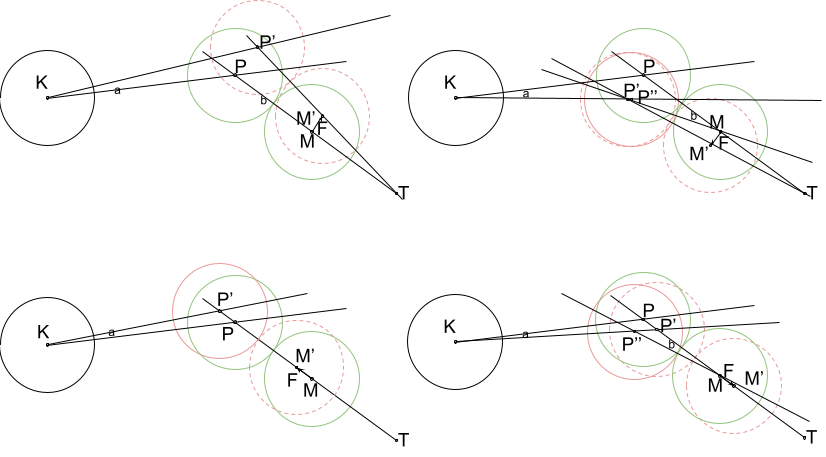
\includegraphics[width=0.5\linewidth]{../common/07_appendix/resources/02_fehlerwinkel.png}
    \end{center}
    \caption{Fehlerwinkel}
    \label{fig:fehlerwinkel}
\end{figure}
Wichtig zu beachten ist auch, dass wenn der Winkel $\beta$ $0$ ist, dies nicht bedeutet,
dass kein Fehler passiert ist. In dem Fall wird die Kugel entweder nicht getroffen (Fehler) oder sie wird korrekt
getroffen (kein Fehler).

Es folgen einige Definitionen, die für die Herleitung von Relevanz sind.
\begin{align}
    T(T_x, T_y), K(K_x, K_y), M(M_x, M_y), M'(M_x', M_y'), F(F_x, F_y)\\
    \vec{TM} = \begin{pmatrix}M_x - T_x\\M_y - T_y\end{pmatrix}, \vec{TM'} = \begin{pmatrix}M_x' - T_x\\M_y' - T_y\end{pmatrix}\\
    \vec{TM_0} = \frac{\vec{TM}}{\norm{\vec{TM}}}\\
    \vec{TM_0'} = \frac{\vec{TM'}}{\norm{\vec{TM'}}}\\
    f(\lambda) = \vec{OM} + \lambda \cdot \vec{TM_0}\\
    f(\lambda)' = \vec{OM'} + \lambda \cdot \vec{TM_0'}\\
    P = f(2R)\\
    P' = f(2R)'
\end{align}

Der Winkel $\beta$ ist also durch Formel \ref{eq:2} gegeben.
\begin{align}
    \cos(\beta) = \frac{\vec{MP} \cdot \vec{MP'}}{\norm{\vec{MP}} \cdot \norm{\vec{MP'}}}\label{eq:2}
\end{align}

Um die maximale Fehlerdistanz zu bestimmen, wird angenommen, dass eine orthogonale Verschiebung des Kugelmittelpunkts
das Worst-Case-Szenario bildet. Dies wird in Abbildung \ref{fig:fehlerwinkel_vereinfachung} verdeutlicht. Es ist nochmals ersichtlich, dass der berechnete Fehlerwinkel $\beta$
nur eine Annäherung darstellt, da der effektive Winkel ein wenig grösser sein wird.
\begin{figure}[h!]
    \begin{center}
        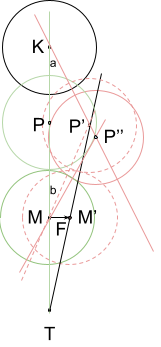
\includegraphics[width=0.2\linewidth]{../common/07_appendix/resources/03_fehlerwinkel_vereinfacht.png}
    \end{center}
    \caption{Fehlerwinkel vereinfacht}
    \label{fig:fehlerwinkel_vereinfachung}
\end{figure}
$M'$ kann nun mittels dem Fehlervektor $\vec{F}$ und $M$ ausgedrückt werden.
\begin{align}
    \vec{M'} = \vec{OM} + \vec{F}\\
    \vec{M'} = \begin{pmatrix}M_x + F_x\\M_y + F_y\end{pmatrix}
\end{align}
Der Punkt $P'$ wird über eine Geradengleichung ausgedrückt, um ihn direkt über den Fehlervektor zu definieren.
\begin{align}
    f(\lambda)' = \vec{OM'} + \lambda \cdot \vec{TM_0'}\\
    TM' = \begin{pmatrix}M_x + F_x - T_x\\M_y + F_y - T_y\end{pmatrix}\\
    TM_0' = \begin{pmatrix}\frac{M_x + F_x - T_x}{\sqrt{(M_x + F_x - T_x)^2 + (M_y + F_y - T_y)^2}}\\\frac{M_y + F_y - T_y}{\sqrt{(M_x + F_x - T_x)^2 + (M_y + F_y - T_y)^2}}\end{pmatrix}\\
    P' = f(2R)' = \begin{pmatrix}M_x + F_x\\M_y + F_y\end{pmatrix} + 2R \cdot \vec{TM_0'}
\end{align}
Der Fehlerwinkel $\beta$ wird nun zwischen den Vektoren $\vec{MP}$ und $\vec{MP'}$ berechnet.
\begin{align}
    \vec{MP} = \begin{pmatrix}M_x + 2R \cdot \frac{M_x - T_x}{\sqrt{(M_x - T_x)^2 + (M_y - T_y)^2}} - M_x\\M_y + 2R \cdot \frac{M_y - T_y}{\sqrt{(M_x - T_x)^2 + (M_y - T_y)^2}} - M_y\end{pmatrix}\\
    \vec{MP} = \begin{pmatrix}2R \cdot \frac{M_x - T_x}{\sqrt{(M_x - T_x)^2 + (M_y - T_y)^2}}\\2R \cdot \frac{M_y - T_y}{\sqrt{(M_x - T_x)^2 + (M_y - T_y)^2}}\end{pmatrix}\label{eq:3}\\
    \vec{MP'} = \begin{pmatrix}(M_x + F_x) + 2R \cdot \frac{M_x + F_x - T_x}{\sqrt{(M_x + F_x - T_x)^2 + (M_y + F_y - T_y)^2}} - M_x\\(M_y + F_y) + 2R \cdot \frac{M_y + F_y - T_y}{\sqrt{(M_x + F_x - T_x)^2 + (M_y + F_y - T_y)^2}} - M_y\end{pmatrix}\\
    \vec{MP'} = \begin{pmatrix}F_x + 2R \cdot \frac{M_x + F_x - T_x}{\sqrt{(M_x + F_x - T_x)^2 + (M_y + F_y - T_y)^2}}\\F_y + 2R \cdot \frac{M_y + F_y - T_y}{\sqrt{(M_x + F_x - T_x)^2 + (M_y + F_y - T_y)^2}}\end{pmatrix}\label{eq:4}
\end{align}
Mittels \ref{eq:3} und \ref{eq:4} kann nun der Fehlerwinkel definiert werden. Der Vektor $\vec{f}$ steht
dabei für den Fehlervektor, welcher zum effektiven Kugelmittelpunkt addiert werden muss. Er wird bei der Lokalisierung von $MP'$
verwendet.
\begin{align}
    \alpha(\vec{f}) = \arccos(\frac{\vec{MP} \cdot \vec{MP'}}{\norm{\vec{MP}} \cdot \norm{\vec{MP'}}})
\end{align}

Um die Auswirkung eines Fehlervektors der Länge $3mm$ darzustellen, wird die vereinfachte Situation aus Abbildung
\ref{fig:fehlerwinkel_vereinfachung} vorausgesetzt. Weiterhin wird verdeutlicht, wie sich die Abweichung $d$ über eine
Distanz $D$ und einen Winkel $\beta$ zusammensetzt. Die Abbildung \ref{fig:abweichung_ueber_distanz} zeigt die Ausgangslage,
wobei $D$ und $\beta$ bekannt sind.
\begin{figure}[h!]
    \begin{center}
        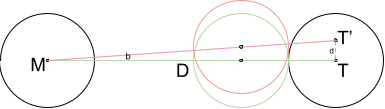
\includegraphics[width=0.4\linewidth]{../common/07_appendix/resources/04_abweichung.png}
    \end{center}
    \caption{Abweichung über Distanz}
    \label{fig:abweichung_ueber_distanz}
\end{figure}
Bei $d$ handelt es sich um die Gegenkathete, bei $D$ um die Ankathete. Daher gelten die Gleichungen \ref{eq:5} und \ref{eq:6}.
\begin{align}
    \cos(\beta) = \frac{D}{Hyp}\\
    \cos(\beta) \cdot Hyp = D\\
    Hyp = \frac{D}{\cos(\beta)}\label{eq:5}\\
    \sin(\beta) = \frac{d}{Hyp}\\
    \sin(\beta) \cdot Hyp = d\\
    Hyp = \frac{d}{\sin(\beta)}\label{eq:6}
\end{align}
Die Formeln \ref{eq:5} und \ref{eq:6} können nun gleichgesetzt und nach $d$ aufgelöst werden. Siehe Formel \ref{eq:7}.
\begin{align}
    \frac{D}{\cos(\beta)} = \frac{d}{\sin(\beta)}\\
    \frac{D \cdot \sin(\beta)}{\cos(\beta)} = d\label{eq:7}
\end{align}

Für eine Abweichung um $\vec{f} = \begin{pmatrix}3\\0\end{pmatrix}$ auf ein Ziel $T$ der Entfernung $T = \begin{pmatrix}0\\-1800\end{pmatrix}$
ergibt sich ein Winkel $\beta$ von $3.378\deg$. Dies ergibt eine Gesamtabweichung von
$\frac{\sin(3.378) \cdot 1800mm}{\cos(3.378)} = 106.251mm$. Es wird davon ausgegangen, dass die Distanzen, welche eine
Kugel zurücklegen, tendenziell kleiner sein werden, da Stösse über grössere Distanzen schwieriger sind. Daher wird die Distanz
auf maximal die halbe Tischlänge gekürzt und die Abweichung sinkt auf $27.31mm$.

Es wird nun eine Länge des Fehlervektors gesucht, der auf eine Distanz von $900mm$ eine Abweichung von $2mm$ zulässt.
Der Winkel ist demnach ca. $0.1273\deg$. Bei einer Fehlervektorlänge von $0.1mm$ ergeben sich $1.82mm$ Abweichung zur
optimalen Bahn.